\documentclass[a4paper,11pt]{article}

% Encoding & fonts
\usepackage[utf8]{inputenc}
\usepackage[T1]{fontenc}
\usepackage{lmodern}

% Language

% Math & symbols
\usepackage{amsmath, amssymb}
\usepackage[polish]{babel}

% Page layout
\usepackage[margin=2.5cm]{geometry}

% Figures
\usepackage{graphicx}

% Clickable links
\usepackage{hyperref}

\begin{document}

\section*{Projekt Shallow Water}
\textit{autor:} Mateusz Cekiera

\textbf{Temat projektu:}
Badanie zjawiska odbicia fali od przeszkody wklęsłej;
\textit{badanie odbicia fali od studni (zamiast ściany) przy pomocy schematu Shallow Water.}

\bigskip

\textbf{Opis projektu:}
Stan początkowy: fala płaska, rozciągająca się wzdłuż osi $y$ i o kształcie krzywej dzwonowej wzdłuż osi $x$, porusza się w dodatnim kierunku osi $x$, w kierunku studni. Parametry początkowe to:
\begin{itemize}
  \item \texttt{grid} – liczba oczek siatki $(X,Y)$,
  \item \texttt{wave\_center}, \texttt{wave\_width}, \texttt{wave\_height} – parametry opisujące położenie i kształt fali; szerokość to parametr odchylenia standardowego krzywej Gaussa,
  \item \texttt{well\_center}, \texttt{well\_width}, \texttt{well\_depth} – parametry opisujące położenie i kształt studni,
  \item $H_0$ – grubość warstwy wody bez zaburzeń,
  \item $g$ – przyspieszenie grawitacyjne.
\end{itemize}

Stan końcowy: dwie fale – pierwotna i odbita, współczynnik $R$ odbicia:
\[
  R = \frac{H_{\mathrm{refl}}}{H_{\mathrm{wave}}},
\]
gdzie $H$ – amplituda fali, refl – fali odbitej, wave – pierwotnej. 

Prędkość początkowa fali to
\[
  u = \sqrt{g H_0},
\]
dla $g = 10.0$, $H_0 = 1.0$. 

\begin{figure}[h]
  \centering
  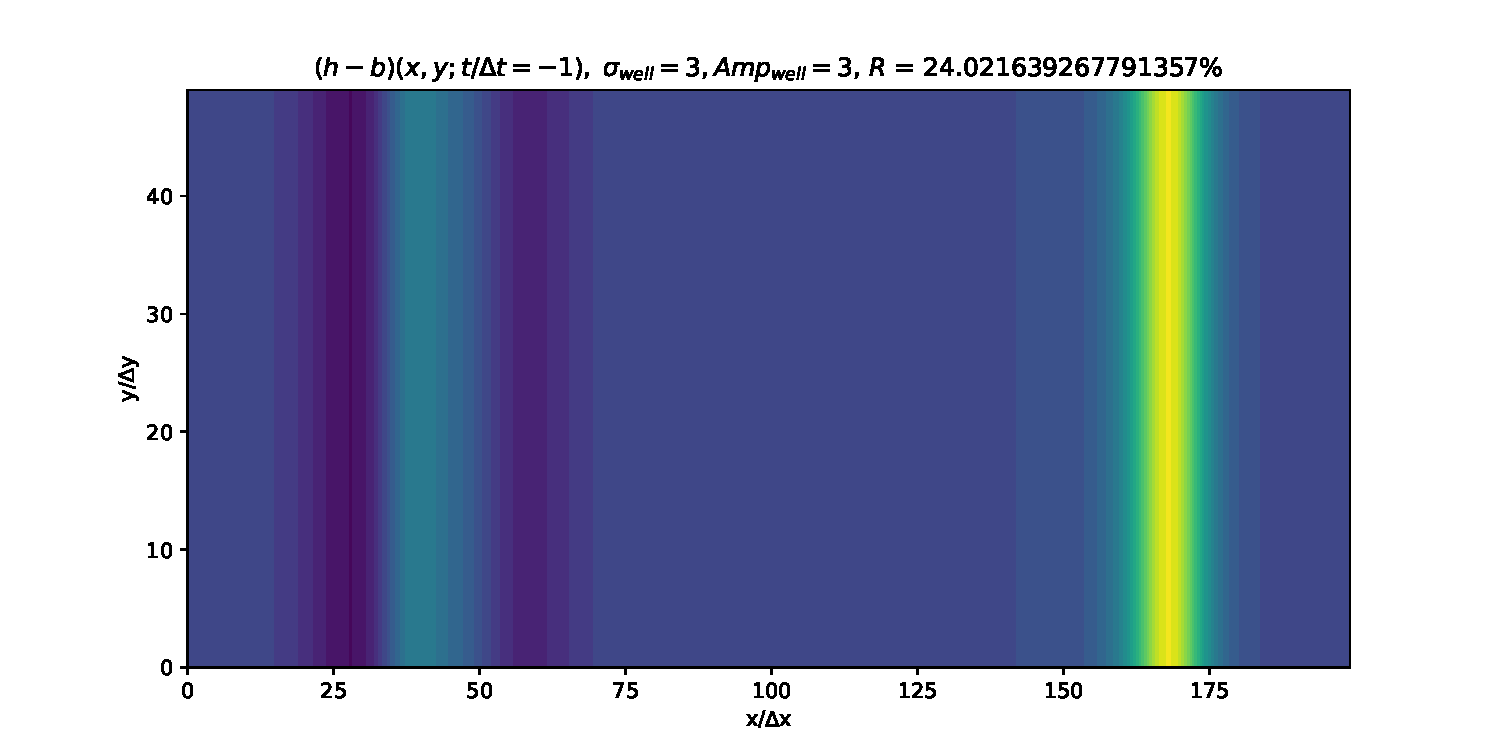
\includegraphics[width=0.8\linewidth]{project_shallow_water/shape.pdf}
  \caption{Kształt fali po odbiciu.}
  \label{fig:shape}
\end{figure}

\begin{figure}[h]
  \centering
  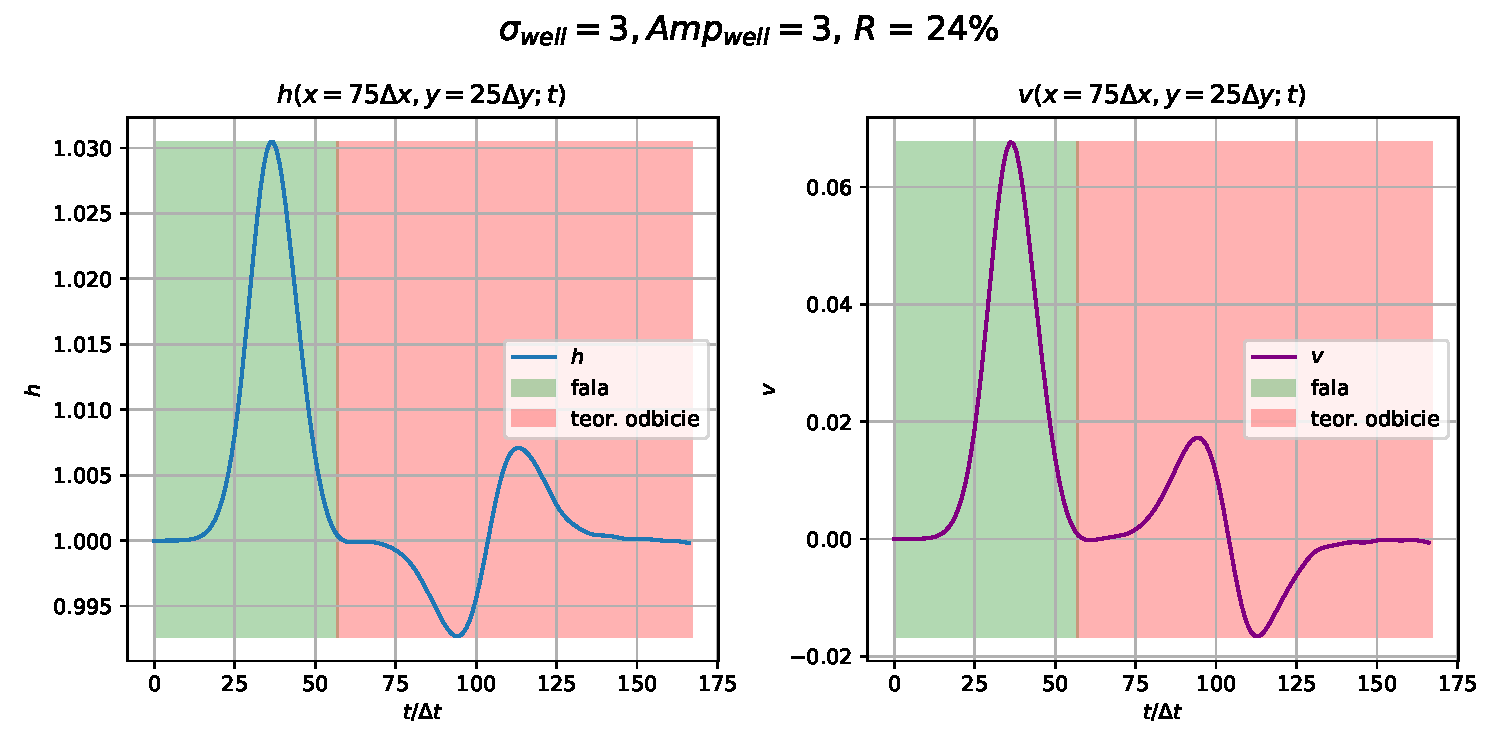
\includegraphics[width=0.8\linewidth]{project_shallow_water/wave_change.pdf}
  \caption{Zależności grubości warstwy i prędkości od czasu.}
  \label{fig:change}
\end{figure}

Do zbadania czynnika $R$ zasymulowano zachowanie fali dla zmiennej grubości studni 
$\sigma_{\mathrm{well}}$ i malejącej amplitudy 
$A_{\mathrm{well}} = \frac{1}{\sigma_{\mathrm{well}}}$. 
W taki sposób objętość studni 
pozostaje taka sama, lecz jej głębokość i szerokość zmieniają się (dla $\sigma\rightarrow 0$ 
wygląda to jak dążenie do delty Diraca). Zakładane to malenie wartości $R$ wraz 
ze wzrostem grubości studni (studnia dąży do kształtu płaskiego), oraz rośnięcie 
dla malejącego $\sigma_{\mathrm{well}}\rightarrow\sigma_{\mathrm{wave}}$. Dla $\sigma_{\mathrm{well}}=\sigma_{\mathrm{well}}$ zakładany jest rezonans i 
maksimum $R$. Poniżej wartość powinna spadać aż do osiągnięcia granicy dokładności 
numerycznej, gdy szerokość studni będzie mniejsza od grubości jednego piksela mapy 
i jej kształ będzie bardziej przypominać pojedynczy abnormalny piksel. 

\begin{figure}[h]
  \centering
  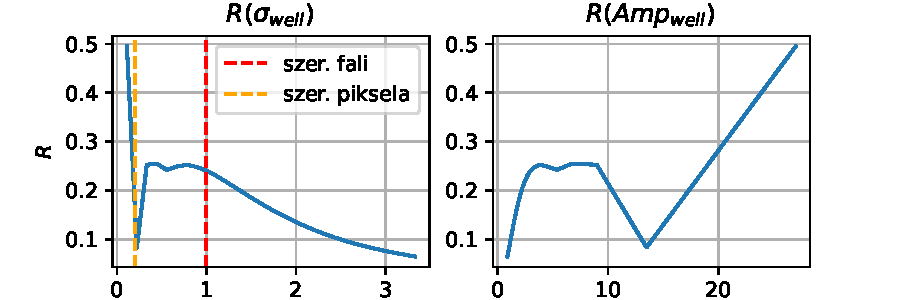
\includegraphics[width=0.8\linewidth]{project_shallow_water/R.pdf}
  \caption{Zależność $R$ od szerokości i amplitudy studni.}
  \label{fig:R}
\end{figure}

\textbf{Test dokładności numerycznej}

Zmniejszono wielkość siatki jak i kroków czasowych do 2/5 (\texttt{grid} = 80x20, \texttt{nt} = 200) 
pierwotnej wartości. Efekt jest również zauważalny. Przy zejściu do 1/5 (\texttt{grid}=40x10, 
\texttt{nt}=100) siatka jest za mała, nakładanie się błędów numerycznych jest za duże aby 
zobaczyć wynik.

\begin{figure}[h]
  \centering
  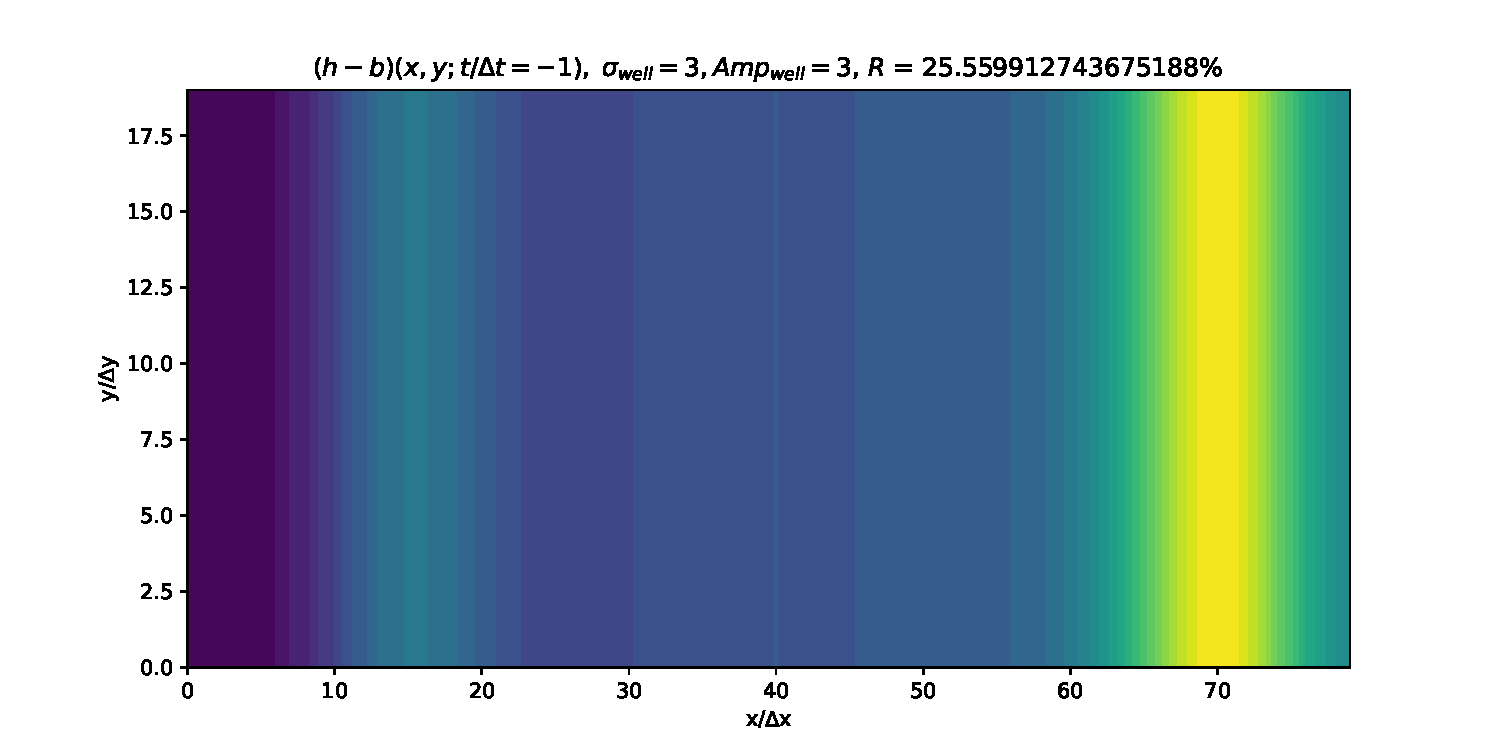
\includegraphics[width=0.8\linewidth]{project_shallow_water/shape_halfresolut.pdf}
  \caption{Kształt fali po odbiciu po zmniejszeniu siatki i kroków czasowych.}
  \label{fig:shape_half}
\end{figure}

\begin{figure}[h]
  \centering
  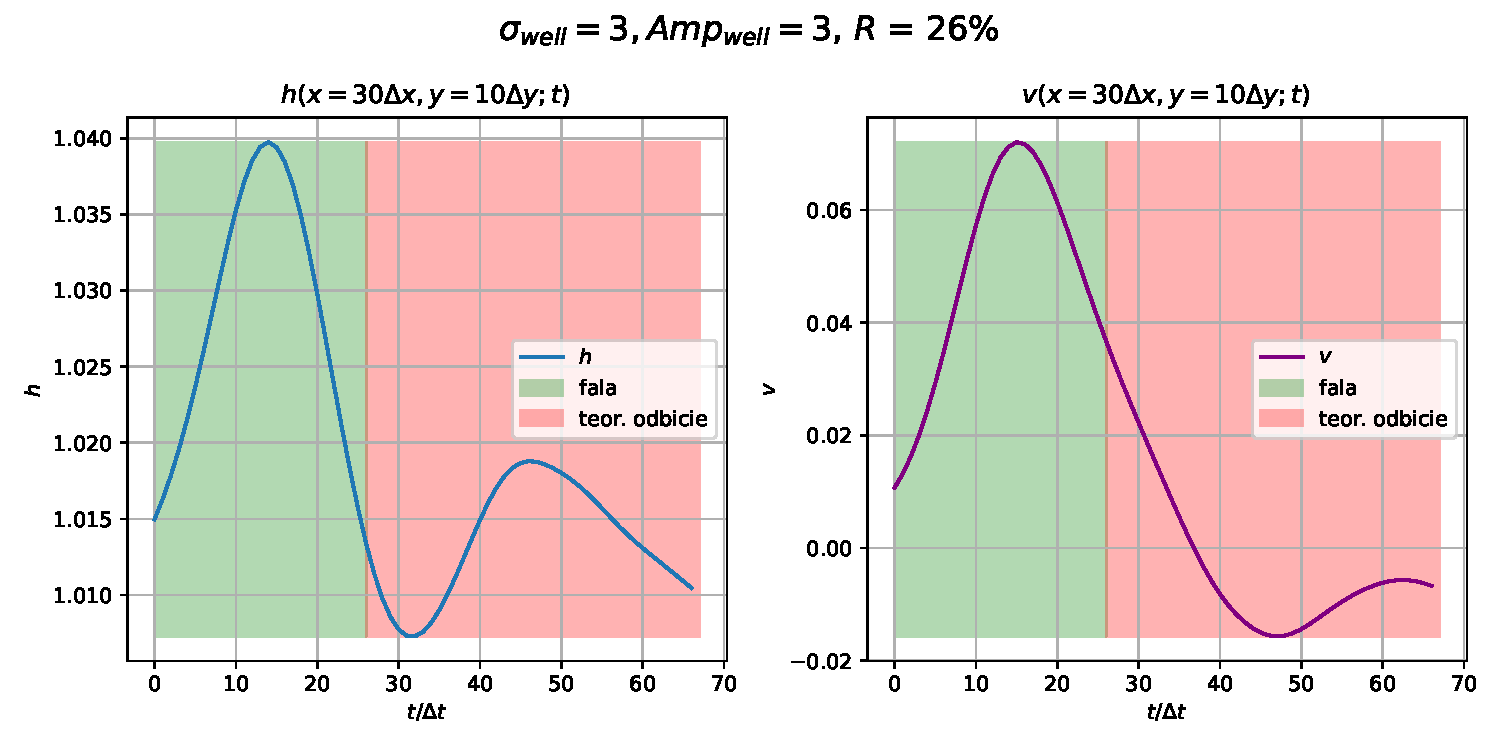
\includegraphics[width=0.8\linewidth]{project_shallow_water/wave_change_halfresolut.pdf}
  \caption{Zależności grubości warstwy i prędkości od czasu po zmniejszeniu siatki i kroków czasowych.}
  \label{fig:change_half}
\end{figure}

Współczynnik $R$ zachowuje się podobnie przy mniejszej rozdzielczości, lecz nagły wzrost związany z limitem dokładności
pojawia się, jak można przewidzieć, przy dwa razy większej wartości niż przy poprzedniej analizie.
\begin{figure}[h]
  \centering
  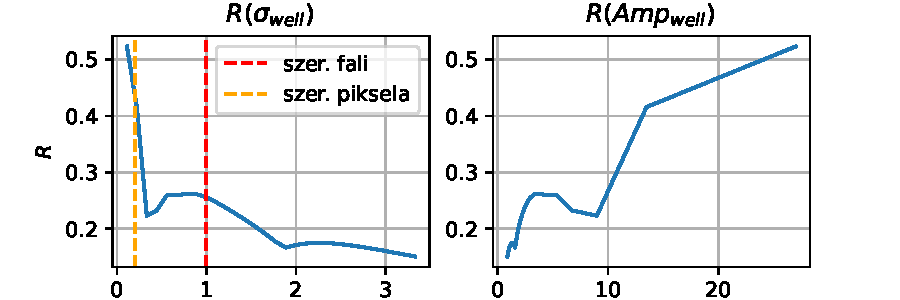
\includegraphics[width=0.8\linewidth]{project_shallow_water/R_half.pdf}
  \caption{Zależność $R$ od szerokości i amplitudy studni po zmniejszeniu rozdzielczości i kroków czasowych.}
  \label{fig:R_half}
\end{figure}

\textbf{Podsumowanie}

Fala może odbić się od wklęsłej przeszkody, a amplituda fali odbitej zależy od 
szerokości i głębokości studni. Im płytsza i szersza studnia, tym niższe *R*. 
Dla głębokich i wąskich studni współczynnik osiąga maksimum około grubości fali,
po czym spada aż do granicy dokładności numerycznej.

\end{document}
